% Created 2019-08-31 sáb 00:03
% Intended LaTeX compiler: pdflatex
\documentclass[11pt]{article}
\usepackage[utf8]{inputenc}
\usepackage[T1]{fontenc}
\usepackage{graphicx}
\usepackage{grffile}
\usepackage{longtable}
\usepackage{wrapfig}
\usepackage{rotating}
\usepackage[normalem]{ulem}
\usepackage{amsmath}
\usepackage{textcomp}
\usepackage{amssymb}
\usepackage{capt-of}
\usepackage{hyperref}
\usepackage[letterpaper,margin=1in,footskip=0.25in]{geometry}
\author{Jorge Francisco Cortés López & Diego Estrada Mejia}
\date{Agosto 30, 2019}
\title{Reporte de conversión de Entidad Relación a tablas\\
  Práctica 3}
\hypersetup{
 pdfauthor={Diego Estrada},
 pdftitle={},
 colorlinks=true,    
 urlcolor=red,
 pdfkeywords={},
 pdfsubject={},
 pdfcreator={Emacs 26.2 (Org mode 9.2.4)}, 
 pdflang={English}}
\begin{document}

\maketitle

\section*{Conversión}
\label{sec:orgd2f6e52}
\begin{center}
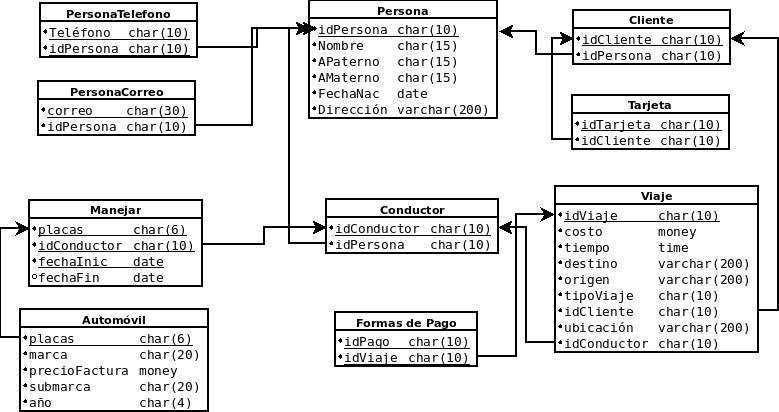
\includegraphics[width=.9\linewidth]{tablas.png}
\end{center}
\section*{Descripción y restricciones}
\label{sec:orge9cb773}
En el diagrama están indicados, por medio de notación, la mayoría de las restricciones
de integridad. Las que falten las indicaremos mas abajo. La notación consta de:
\begin{itemize}
\item \textdegree{} el atributo puede ser \texttt{null}
\item \textbullet{} el atributo no puede ser \texttt{null}
\item \uline{atributo} si el atributo está subrayado y con un rombo al inicio es una llave primaria 
(o parte de una llave compuesta).
\end{itemize}
Indicaremos, tabla por tabla las restricciones que faltan, junto con la explicación de los dominios
de cada atributo y de las referencias de sus llaves. Además en las relaciones que
surgieron de la conversión haremos una descripción de estas.
\subsection*{Persona}
\label{sec:org247eb51}
\begin{itemize}
\item \textbf{idPersona} tiene como dominio \texttt{char(10)} porque pensamos que un identificador de 10 carácter para cada persona
que se registre es suficiente. Esta misma decisión se tomó para todos los identificadores de la base de 
datos.
\item \textbf{Nombre} tiene como dominio \texttt{char(15)} porque un nombre es una cadena de carácteres de una longitud medianamente larga.
\item \textbf{APaterno} tiene como dominio \texttt{char(15)} porque un apellido es una cadena de carácteres.
\item \textbf{AMaterno} lo mismo que APaterno.
\item \textbf{FechaNac} tiene como dominioa \texttt{date} pues queremos guardar la fecha de nacimiento.
\item \textbf{Dirección} tiene como dominio \texttt{varchar(200)} pues una dirección a veces puede ser muy simple o puede ser una cadena
bastante larga, el límite es porque pensamos que ninguna dirección supera los 200 carácteres.
\end{itemize}
\subsection*{Viaje}
\label{sec:org36ac98a}
\begin{itemize}
\item \textbf{idViaje} tiene como dominio \texttt{char(10)} pues es un identificador.
\item \textbf{costo} tiene como dominio \texttt{money} pues aqui guardaremos el precio de cada viaje.
\item \textbf{tiempo} tiene como dominio \texttt{time} pues guardaremos el tiempo que tardó cada viaje.
\item \textbf{destino} tiene como dominio \texttt{varchar(200)} pues al igual que la dirección en \emph{Persona} puede ser una cadena muy larga.
\item \textbf{origen} lo mismo que destino.
\item \textbf{tipoViaje} tiene como dominio \texttt{char(10)} porque el nombre de ningún tipo de viaje rebasa los 10 carácteres.
\item \textbf{idCliente} es una llave foránea de \emph{Cliente}, esto porque cada valor en esta tabla debe tener una tupla
en la tabla que refiera a un cliente específico. Como es una llave foránea debe tener el mismo dominio que el valor al que referencia.
\item \textbf{ubicación} tiene como dominio \texttt{varchar(200)} pues es una ubicación.
\item \textbf{idConductor} es una llave foránea de \emph{Conductor}, por lo tanto tiene el mismo dominio que el valor al que referencia.
\end{itemize}
\subsection*{Automóvil}
\label{sec:org15c4b37}
\begin{itemize}
\item \textbf{placas} tiene como dominio \texttt{char(7)} pues son cadenas de carácteres con a lo más 7 letras.
\item \textbf{marca} tiene como dominio \texttt{char(20)} pues el nombre de las marcas de carro normalmente no es tan largo.
\item \textbf{precioFactura} tiene como dominio \texttt{money} pues es el precio del auto.
\item \textbf{submarca} tiene como dominio \texttt{char(20)} pues normalmente el nombre de las submarcas no son largo.
\item \textbf{año} tiene como dominio \texttt{char(4)} pues solo guardaremos los 4 digitos del año.
\end{itemize}
\subsection*{Manejar}
\label{sec:org532cd8d}
\begin{itemize}
\item \textbf{placas} es una llave foránea de \emph{Automóvil}, por lo que comparten dominios.
\item \textbf{idConductor} es una llave foránea de \emph{Conductor}, comparten dominios.
\item \textbf{fechaInic} es una \texttt{date} pues es la fecha en la que el conductor empezó a viajar con el carro específico.
\item \textbf{fechaFin} es una \texttt{date} por el mismo motivo que la fechaInic.
\end{itemize}
\subsection*{Conductor}
\label{sec:org20d51d3}
\begin{itemize}
\item \textbf{idConductor} es un \texttt{char(10)} pues es un identificador.
\item \textbf{idPersona} es llave foránea que referencia a un atributo de \emph{Persona}, por lo que comparten atributos.
\end{itemize}
\subsection*{PersonaTeléfono}
\label{sec:org687c26c}
Ésta relación es nueva gracias a la conversión, necesitamos representar que el atributo teléfono en \emph{Persona} es
multivaluado
\begin{itemize}
\item \textbf{Teléfono} es un \texttt{char(10)} pues los números de teléfono son de esa longitud.
\item \textbf{idPersona} es una llave foránea de \emph{Persona}, por lo que comparte dominio con el atributo que referencia.
\end{itemize}
\subsection*{PersonaCorreo}
\label{sec:org888d119}
Otra relación nueva por la conversión que necesitamos porque podemos tener varios correos.
\begin{itemize}
\item \textbf{correo} es un \texttt{char(30)} porque creemos que es una longitud adecuada para cualquier correo electrónico.
\item \textbf{idPersona} es una llave foránea de \emph{Persona}, comparte dominio con el atributo al que referencia.
\end{itemize}
\subsection*{Formas de Pago}
\label{sec:orgc0a70e7}
Ésta relación se formó en la conversión pues el atributo forma de pago de \emph{Viaje} es multivaluado, por lo que
necesitamos crear una nueva relación.
\begin{itemize}
\item \textbf{idPago} es un identificador, por lo que tiene dominio \texttt{char(10)}.
\item \textbf{idViaje} es una llave foránea de \emph{Viaje}, por lo que comparte el dominio del identificador.
\end{itemize}
\subsection*{Cliente}
\label{sec:org9c372e5}
\begin{itemize}
\item \textbf{idCliente} es un identificador, por lo que tiene dominio en \texttt{char(10)}.
\item \textbf{idPersona} es una llave foránea de \emph{Persona}, comparten dominios.
\end{itemize}
\subsection*{Tarjeta}
\label{sec:org542e61c}
\begin{itemize}
\item \textbf{idTarjeta} es un identificador, por lo que su dominio es \texttt{char(10)}.
\item \textbf{idCliente} es una llave foránea de \emph{Cliente}, comparte dominios con el identificador.
\end{itemize}

\section*{Preguntas.}
\begin{enumerate}
    \item ¿Cuáles son las principales diferencias entre el diagrama E-R y Relacional?\\
    La diferencia principal entre el diagrama E-R y relacional es que el diagrama E-R se enfoca entre las entidades y sus relaciones. Por otro lado, el modelo relacional se enfoca en tablas y la relación entre los datos de las tablas.\\
    Un diagrama E-R describe los datos con el conjunto de entidades, relaciones y atributos. Sin embargo, el modelo relacional describe los datos con las tuplas, atributos y el dominio de los atributos.\\
    Uno puede entender fácilmente las relaciones entre los datos en el diagrama E-R comparado con el modelo relacional.\\
    El diagrama E-R tiene una cardinalidad asociada como una restricción en donde el modelo relacional no tiene esa restricción.
    
    \item ¿Cuáles son las principales características del diagrama E-R?
    Un diagrama E-R es una representación gráfica que modela relaciones entre personas, objetos, conceptos o eventos dentro de un sistema.
    Existen cinco componentes básicos de un diagrama entidad-relación.
    Componentes similares estarán diseñados por la misma forma. Por ejemplo, todas las entidades estarán encerradas por un rectangulo, mientras que todos los atributos estarán encerrados por un rombo. Las componentes incluyen:\\
    \begin{enumerate}
        \item Entidades, las cuales son objetos o conceptos que pueden tener datos guardados sobre ellos. Las entidades se refieren a las tablas que usamos en las BDD.
        \item Atributos, los cuales son propiedades o características de las entidades. Un atributo puede ser denotado como una llave primaria, la cual identifica un atributo único, o una llave foránea, la cual puede ser asignada a múltiples atributos.
        \item Las relaciones entre y sobre esas entidades
        \item Acciones, las cuales describen como las entidades comparten información a la base de datos.
        \item Conexión de líneas.
    \end{enumerate}
    Una notación de cardinalidad puede entonces definir los atributos de la relación entre las entidades. Las cardinalidades pueden denotar que una entidad es opcional (Por ejemplo, un cliente puede o no tener una tarjeta de cliente distinguido) u obligatoria (Por ejemplo, debe haber al menos un producto listado en un almacen).\\
    Las tres principales cardinalidades son:
    \begin{enumerate}
        \item Una relación uno-a-uno (1:1). Por ejemplo, si cada cliente en una bases de datos está asociado con una sola dirección de envío.
        \item Una relación uno a varios (1:M). Por ejemplo, un sólo cliente puede hacer una orden para múltiples productos. El cliente está asociado con varias entidades, pero todas esas entidades tienen una sola conexión de regreso con el mismo cliente.
        \item Una relación de varios a varios (M:N). Por ejemplo, una compañia en donde todos los agentes del call center trabajan con múltiples clientes, cada agente está asociado con varios clientes, y varios clientes pueden estar relacionados con muchos otros agentes.
    \end{enumerate}
    
    \item ¿Es necesario tener llaves primarias en cada entidad de nuestro diagrama? Explica.\\
    Las llaves primarias y foráneas son una manera en las cuales podemos restringir datos relacionados para asegurarnos que la BDD se mantenga consistente y para asegurarnos de que no hayan datos redundantes en la BDD como resultado de eliminar una tabla o una columna en una de las tablas que puede afectar los datos en otras tablas que puedan estar relacionadas. Puede causar problemas de integridad de datos así como problemas en la aplicación que haga uso de la base de datos. Por lo que siempre es recomendable asignar una llave primaria o foránea a cada entidad.
    
    \item Explica con tus palabras que es una llave primaria (PK), llave candidata (UNIQUE) y llave foránea (FK)\\
    \textbf{PK} Una llave primaria es un atributo o conjunto de atributos que nos ayudan a identificar un ejemplar de una entidad, una llave primaria en general debería de cumplir con:\\
    Tener un valor no vacío para cada ejemplar de la entidad, el valor debe ser único para cada ejemplar de la entidad y los valores no deben cambiar o convertirse en vacíos a lo largo de la existencia de los ejemplares de la entidad.\\
    \textbf{UNIQUE} Una llave candidata es una combinación de atributos que pueden ser usados únicamente para identificar un ejemplar de la entidad sin referirse a otros datos. Todas las llaves candidatas tienen algunas propiedades en común. Una de las propiedades es que durante la existencia de la llave candidata, el atributo usado para la identificación debe mantenerse igual, luego otra propiedad es que el valor no puede ser vació y que además la llave candidata debe ser única.\\
    \textbf{FK} Una llave foránea es un atributo que completa una relación identificando la entidad padre. Las llaves foráneas proveen un método para mantener la integridad de los datos (llamada integridad referencial) y para navegar entre diferentes instancias de una entidad. Cada relación en el modelo debe estar sostenidad por una llave foránea.
\end{enumerate}

\section*{Tabla de tipos de datos.}
A continuación se muestra una tabla con los diferentes tipos de datos con los que cuenta PostegreSQL.Se pueden consultar en la \href{https://www.postgresql.org/docs/9.2/datatype.html}{documentación}.

\begin{center}
\begin{tabular}{ |c|c|c|  }
 \hline
 \multicolumn{3}{|c|}{Lista de tipos de datos en PostegreSQL} \\
 \hline
Nombre de tipo & Alias & Descripción\\
\hline
bigint & int8 & entero de 8 bits con signo\\
\hline
bigserial & serial8 & entero de 8 bits auto-incrementante\\
\hline
bit [ (n) ] &  & cadena de bits de tamaño fijo\\
\hline
bit varying [ (n) ] & varbit &  cadena de bits de tamaño variable\\
\hline
boolean & bool & valor booleano\\
\hline
box & & caja rectangular en un plano\\
\hline
bytea & & datos binarios ("arreglo de bytes")\\
\hline
character [ (n) ] & char [ (n) ]& cadena de caractéres de tamaño fijo\\
\hline
character varying [ (n) ] & varchar [ (n) ] & cadena de caractéres de tamaño variable \\
\hline
cidr & & dirección de red IPv4 o IPv6\\
\hline
circle & & círculo en un plano\\
\hline
date & & fecha de calendario (año, mes, día)\\
\hline
double precision & float8 & número real con doble precisión\\
\hline
inet & & dirección host IPv4 o IPv6\\
\hline
integer & int, int4 & entero de cuatro bits con signo\\
\hline
interval [fields] [(p)] && Intervalo de tiempo\\
\hline
json && dato JSON\\
\hline
line && linea infinita en un plano\\
\hline
lseg && segmento de linea en un plano\\
\hline
macaddr && dirección MAC\\
\hline
money && valor monetario\\
\hline
numeric [(p,s)] & decimal [(p,s)] & selección precisa de un valor numérico\\
\hline
path && trayectoria geométrica en un plano\\
\hline
point && punto geométrico en un plano\\
\hline
polygon && trayectoria cerrada en un plano\\
\hline
real & float4 & número real con precisión simple\\
\hline
smallint & int2 & entero con signo de dos bytes\\
\hline
smallserial & serial2 & entero autoincrementante de dos bytes\\
\hline
serial & serial4 & entero autoincrementante de cuatro bytes\\
\hline
text && cadena de tamaño variable\\
\hline
time [(p)] [without time zone] && tiempo del día (sin zona horaria)\\
\hline
time [(p)] with time zone & timetz & tiempo del día. con zona horaria\\
\hline
timestamp [(p)] [without time zone] && fecha y hora (sin zona horaria)\\
\hline
tsquery && consulta de texto\\
\hline
tsvector && búsqueda de texto en documento\\
\hline
txid\_snapshot && ID de transacción a nivel de usuario de una copia\\
\hline
uuid && identificador único universal\\
\hline
xml && dato XML\\
 \hline
\end{tabular}
\end{center}


\end{document}
